\documentclass{article}

\usepackage{graphicx}
\usepackage{tikz}
\usepackage{tikzsymbols}
\usetikzlibrary{calc,patterns,shapes.geometric}
\pagestyle{empty}
\usepackage[margin=0pt]{geometry}
\geometry{papersize={14in,12in}}

\def\centerarc[#1](#2)(#3:#4:#5){\draw[#1] ($(#2)+({#5*cos(#3)},{#5*sin(#3)})$) arc (#3:#4:#5);}

\begin{document}
	\begin{figure}
		\centering
		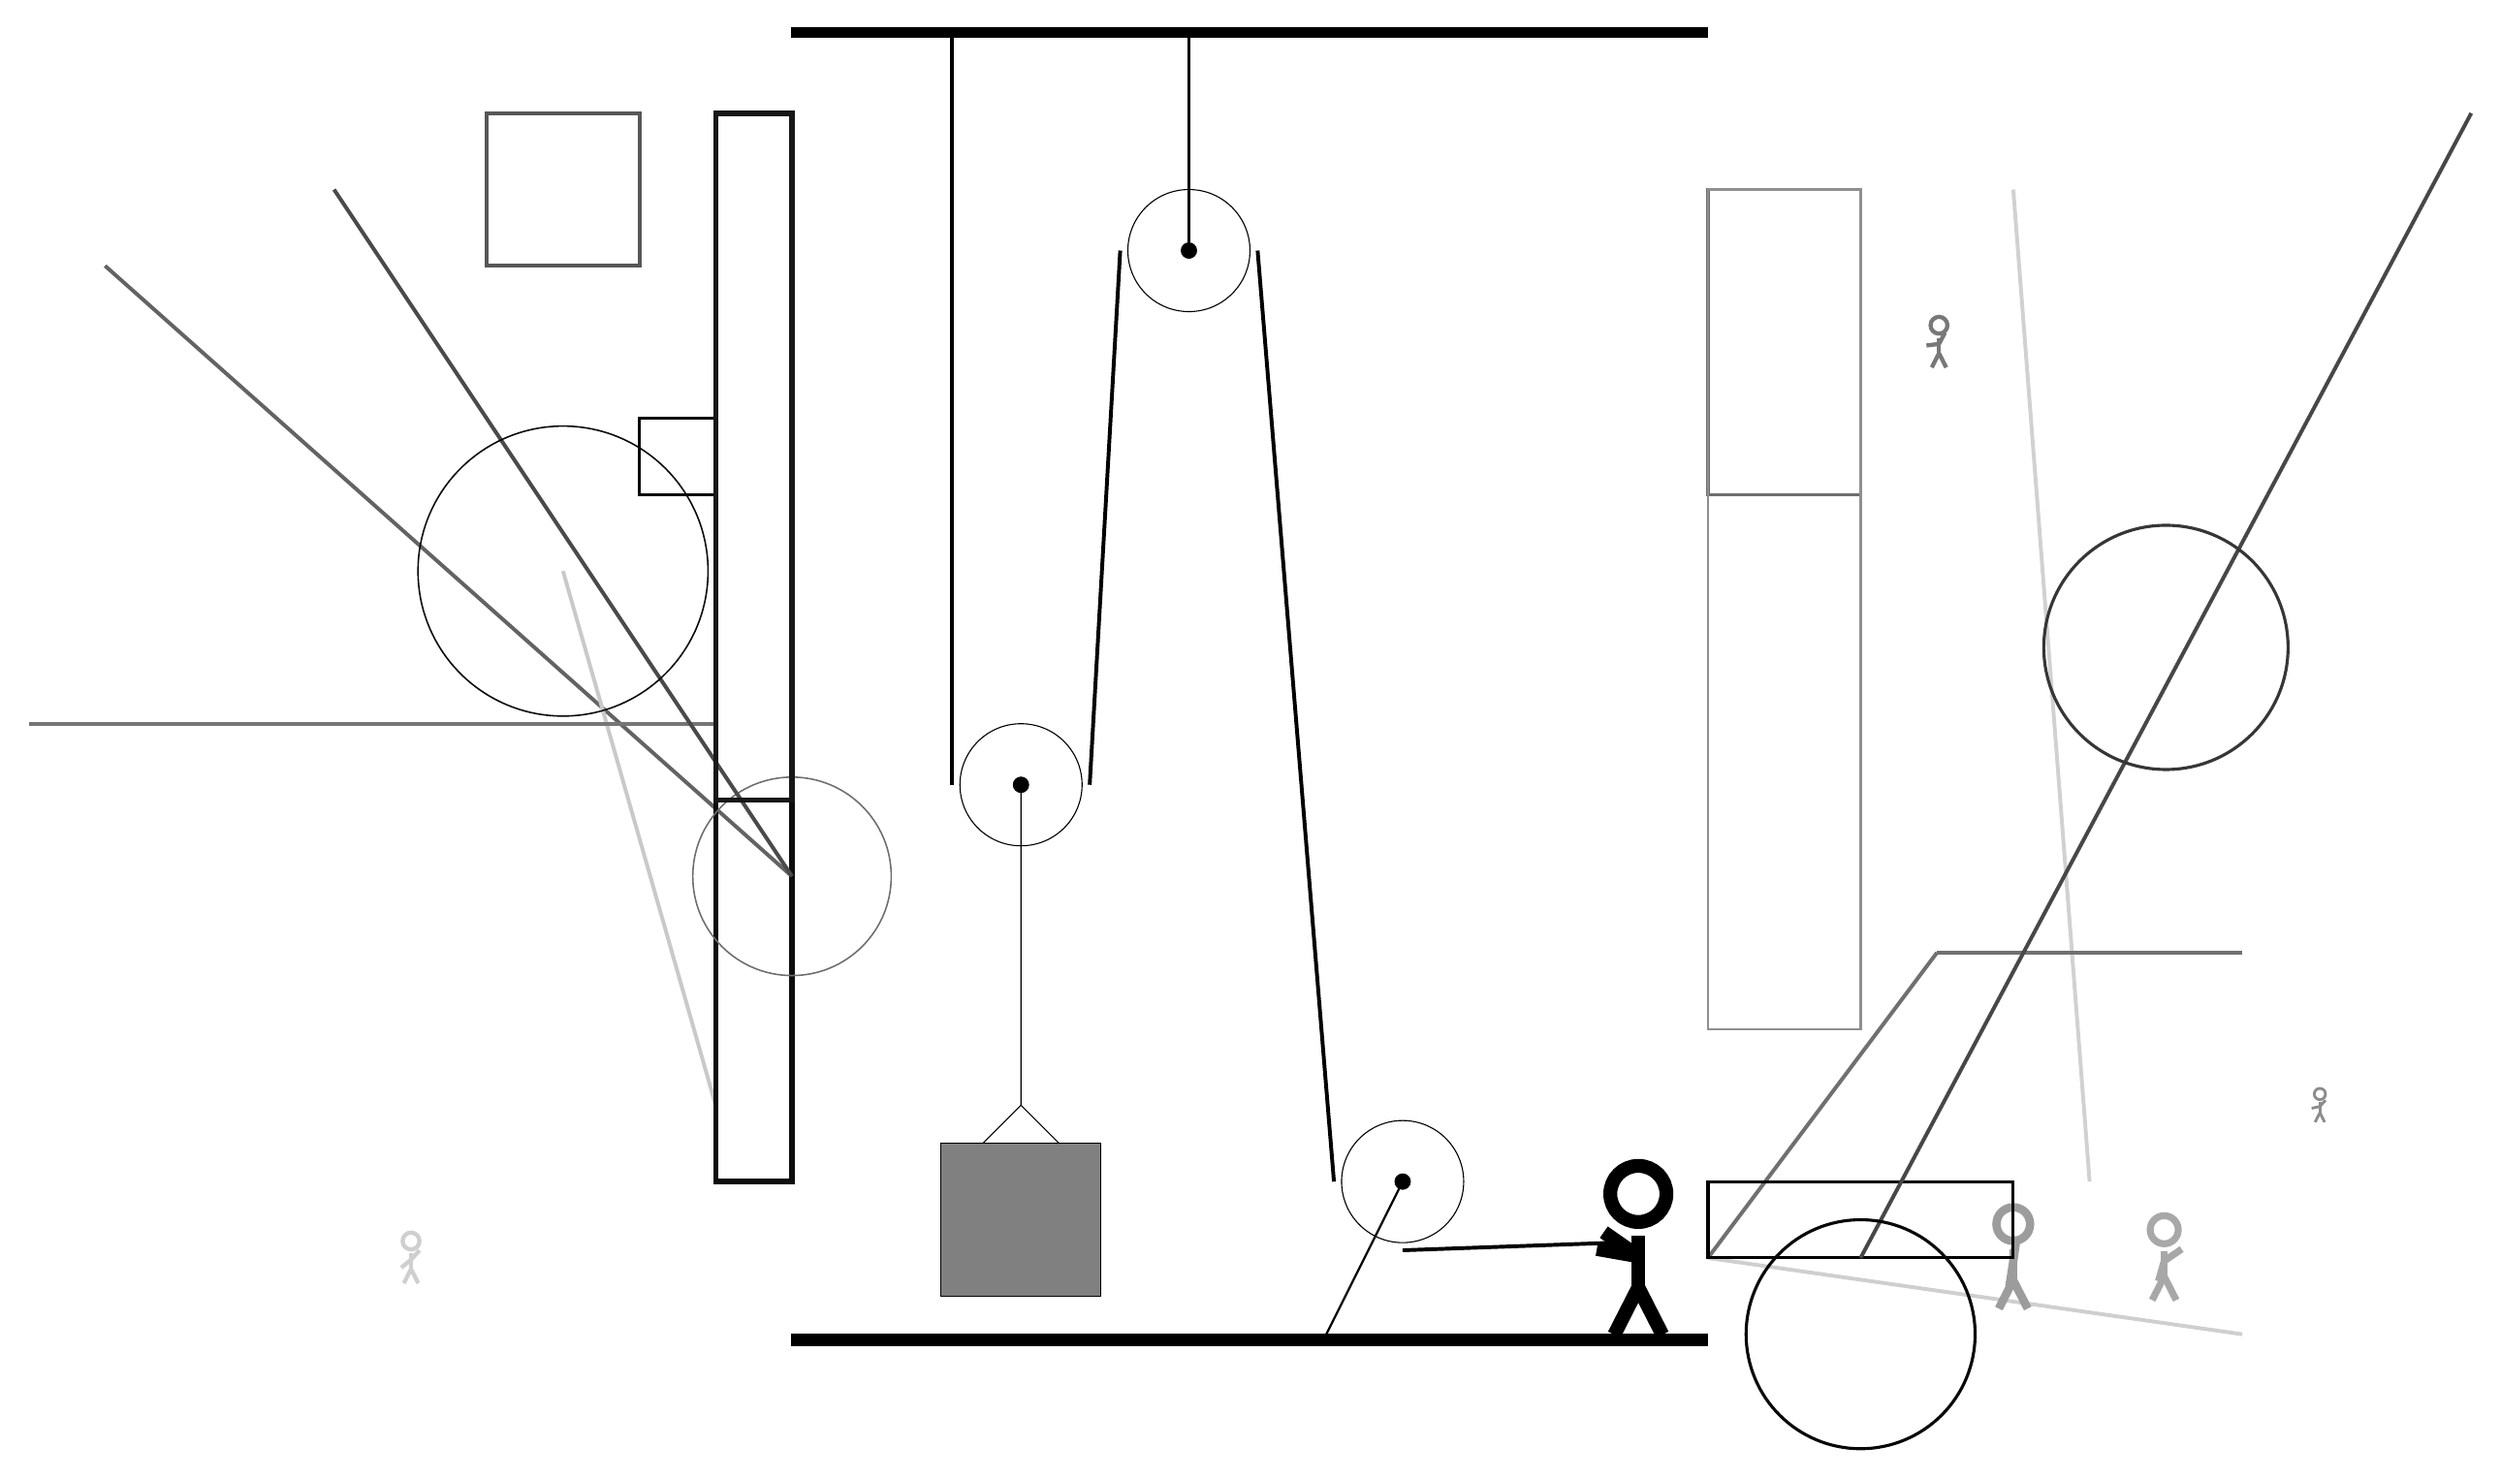
\begin{tikzpicture}
			%%%%% START %%%%%
			
			\draw[fill=black] (-2, 14) rectangle (10, 14.125);
			
			\draw (3.2, 11.2) circle (0.8);
			\draw[fill=black] (3.2, 11.2) circle (0.1);
			\draw[thick] (3.2, 11.2) -- (3.2, 14);
			
			\draw (6, -1) circle (0.8);
			\draw[fill=black] (6, -1) circle (0.1);
			\draw[thick] (6, -1) -- (5, -3);
			
			\draw (1, 4.2) circle (0.8);
			\draw[fill=black] (1, 4.2) circle (0.1);
			
			\draw[line width=0.5mm, color=black!56](13, 2) -- (10, -2);
			
			\draw[line width=0.5mm, color=black!18](15, -1) -- (14, 12);
			\draw[line width=0.2mm, color=black!99] (-3, -2) rectangle (-3, -2);
			\draw[line width=0.5mm, color=black!61](-2, 3) -- (-11, 11);
			
			\draw[line width=0.5mm, color=black!56](13, 2) -- (17, 2);
			
			\draw[line width=0.5mm, color=black!19](10, -2) -- (17, -3);
			\node[line width=0.4mm, color=black!39] at (14, -2) {\Strichmaxerl[6][81][82]};
			
			\draw[line width=0.5mm, color=black!21](-5, 7) -- (-3, 0);
			\draw[line width=0.7mm, color=black!95] (-3, -1) rectangle (-2, 13);
			\draw [line width=0.2mm, color=black!57](-2, 3) circle (1.3);
			\draw[line width=0.5mm, color=black!54](-3, 5) -- (-12, 5);
			\draw[line width=0.4mm, color=black!100] (10, -2) rectangle (14, -1);
			\draw[line width=0.5mm, color=black!66] (-4, 13) rectangle (-6, 11);
			
			\draw[line width=0.5mm, color=black!71](-2, 3) -- (-8, 12);
			\draw[line width=0.4mm, color=black!57] (10, 8) rectangle (12, 12);
			\draw [line width=0.2mm, color=black!97](-5, 7) circle (1.9);
			
			\draw[line width=0.5mm, color=black!72](12, -2) -- (20, 13);
			
			\draw [line width=0.4mm, color=black!97](12, -3) circle (1.5);
			\draw [line width=0.4mm, color=black!79](16, 6) circle (1.6);
			
			\node[line width=0.6mm, color=black!19] at (-7, -2) {\Strichmaxerl[3][39][48]};
			\node[line width=0.6mm, color=black!53] at (13, 10) {\Strichmaxerl[3][7][62]};
			
			\draw[line width=0.4mm, color=black!97] (-4, 8) rectangle (-3, 9);
			
			\draw[line width=0.3mm, color=black!44] (10, 1) rectangle (12, 12);
			\node[line width=0.7mm, color=black!34] at (16, -2) {\Strichmaxerl[5][74][34]};
			\node[line width=0.5mm, color=black!45] at (18, 0) {\Strichmaxerl[2][12][48]};
			\draw[line width=0.7mm, color=black!91] (-3, 4) rectangle (-2, 13);
			
			\draw (1, 4.2) -- (1, 0) -- (0.5, -0.5);
			\draw (1, 0) -- (1.5, -0.5);
			\draw[fill=black!50] (-0.05, -0.5) rectangle (2.05, -2.5);
			
			\draw[line width=0.5mm] (0.1, 14) -- (0.1, 4.2);
			\centerarc[line width=0.5mm](1, 4.2)(180:360:0.9);
			\draw[line width=0.5mm](1.9, 4.2) -- (2.3, 11.2);
			\centerarc[line width=0.5mm](3.2, 11.2)(0:180:0.9);
			\draw[line width=0.5mm](4.1, 11.2) -- (5.1, -1);
			\centerarc[line width=0.5mm](6, -1)(180:270:0.9);
			\draw[line width=0.5mm](6, -1.9) -- (8.8, -1.8);
			
			\node at (9, -1.9) {\Strichmaxerl[10][-35][170]};
			
			\draw[fill=black] (-2, -3) rectangle (10, -3.15);
			
			%%%%% END %%%%%
		\end{tikzpicture}
	\end{figure}	
\end{document}